
\begin{columns}[T]
    \begin{column}{.33\linewidth}
        \begin{itemize}
            \item 高分子材料の破壊耐性向上の設計指針
            \item 耐久性、可逆性に優れたゴム材料
            \item 破壊工学的$\Rightarrow$クラック進展を抑制
        \end{itemize}
        \centering
        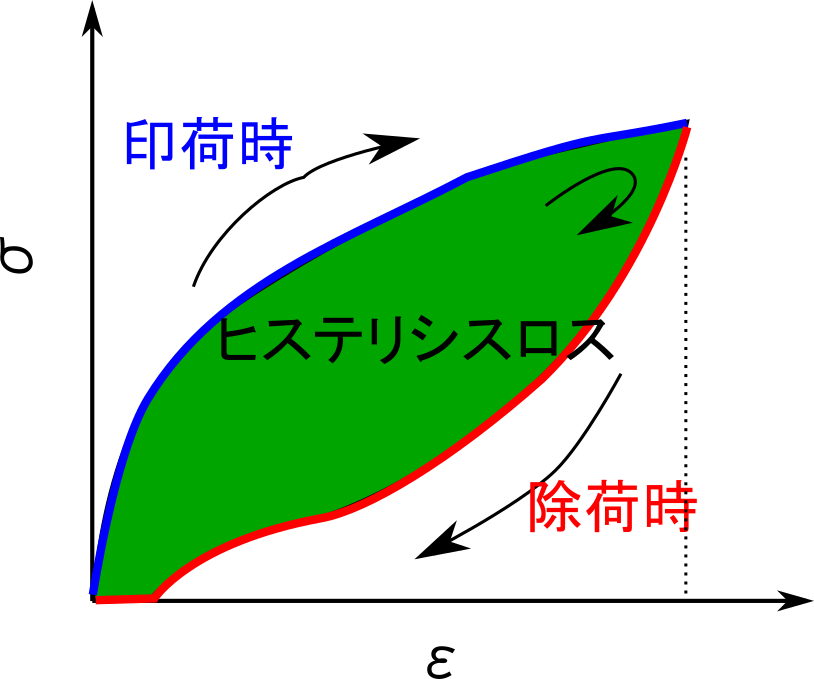
\includegraphics[width=.4\textwidth]{hysteresis_curve.png} 
    \end{column}
    \begin{column}{.33\linewidth}
        \begin{itembox}[l]{Andrews 理論\cite{andrews}}
            \begin{columns}[totalwidth=.9\textwidth]
                \column{.8\textwidth}
                    クラックの微小進展時に、
                    \begin{itemize}
                    \item
                    \textcolor{blue}{Loading 場とUnloading 場}
                    \item
                    \alert{この差}が、全体の変形に要したエネルギーを\alert{散逸}
                    \item
                    鎖破断のエネルギーが低減 $\Rightarrow$ \alert{強靭さの起源。}
                    \end{itemize}	
                \column{.2\textwidth}
                    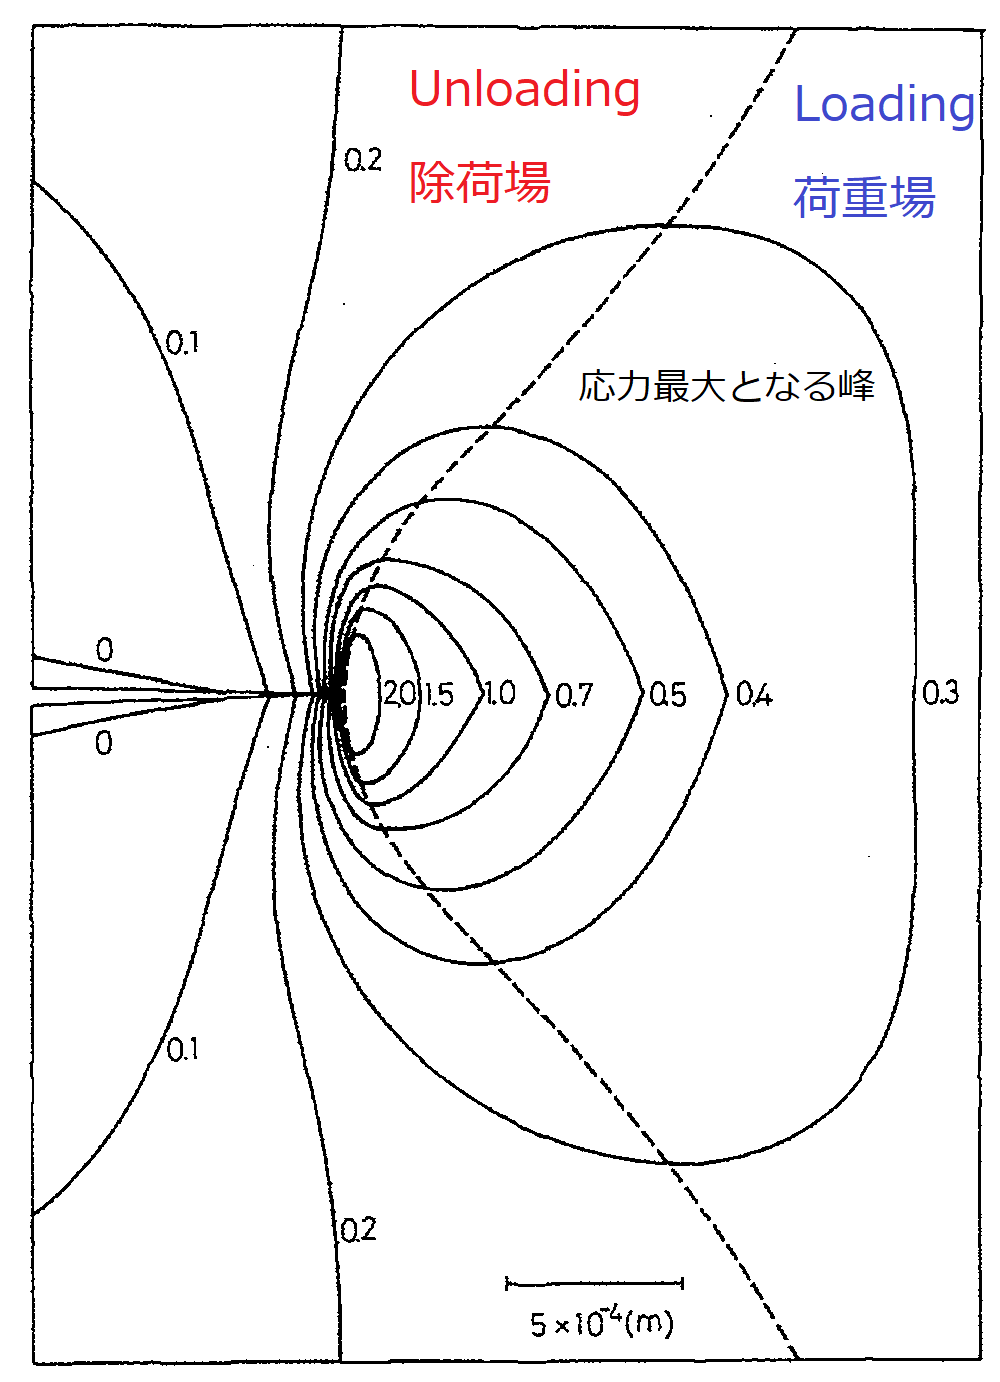
\includegraphics[width=\textwidth]{crack.png}     
            \end{columns}
        \end{itembox}
    \end{column}
    \begin{column}{.33\linewidth}
        \begin{itembox}[l]{ランダム構造とは?}
            \begin{columns}[totalwidth=.9\textwidth]
                \column{.6\textwidth}
                        \begin{itemize}
                            \item 連結性を不均一に
                                \begin{itemize}
                                    \item 連結に\alert{位置依存性}
                                \end{itemize}
                            \item 巨視的な変形後
                                \begin{itemize}
                                    \item 結節点のゆらぎが不均一
                                    \item 多様な緩和モード
                                    % \item \alert{緩和の長時間化?}
                                % \item ファントムネットワークモデルの諸特性の発現?
                                \end{itemize}
                            % \item \alert{解析を容易}に、
                            % 	\begin{itemize}
                            % 		\item 既往研究で反応系
                            % 		\item ストランド長と結合数を一定
                            % 	\end{itemize}
                        \end{itemize}
                \column{.3\textwidth}
                    % ランダム構造の模式図
                    % \vspace{10mm}
                    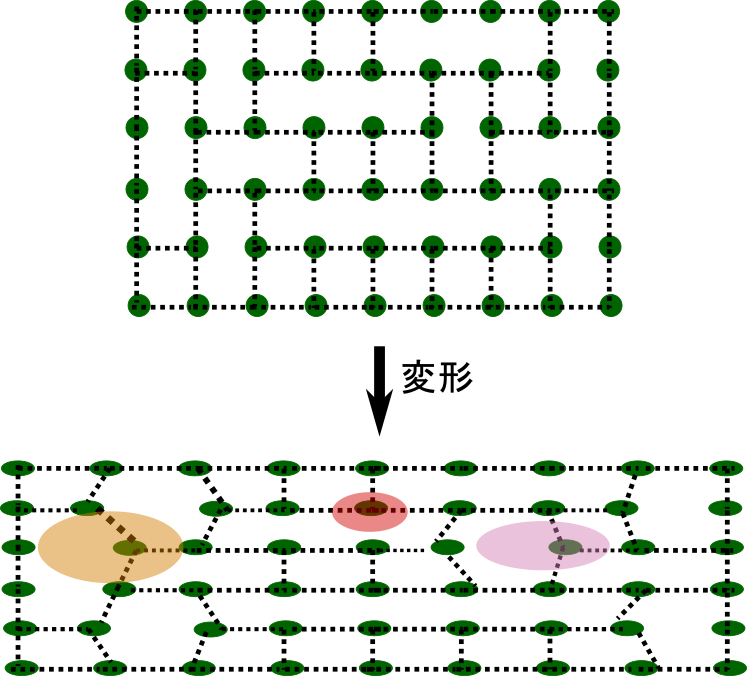
\includegraphics[width=\textwidth]{random_NW.png}
            \end{columns}
        \end{itembox}
    \end{column}
\end{columns}